\chapter[Annual Variation of Coastal Uplift in Greenland as an Indicator of Variable and Accelerating Ice Mass Loss]{Annual Variation of Coastal Uplift in Greenland as an Indicator of Variable and Accelerating Ice Mass Loss \footnote{This chapter has been reprinted from Geochemistry Geophysics Geosystems with permission as: Yang, Q., Wdowinski S., Dixon, T. H., (2013), Annual variation of coastal uplift in Greenland as an indicator of variable and accelerating ice mass loss, Geochem. Geophys. Geosyst., 14, 1569–1589, doi:10.1002/ggge.20089.}}

\section{Abstract} 
Seasonal melting of the coastal part of the Greenland ice sheet is investigated using GPS vertical displacement data from coastal stations, combined with data on atmospheric and ocean temperatures.
Using a high pass filter and cubic spline models, we estimate five variables describing seasonal uplift, a proxy for proximal mass loss, including duration of the melt season and the amount of summer uplift. Our analysis shows both temporal and spatial variations of uplift. Southern coastal Greenland experienced
anomalously large uplift in summer 2010, implying significant melting that year. However, the northwest coast did not experience significant change in uplift at that time. Our data suggest that a combination of warm summer air temperature and warm sub-surface ocean water temperature drove the large mass losses in 2010. Using the uplift pattern of 2008–2010, and comparing to atmospheric data and ocean water temperature data, we show that warm Irminger Water (IW) exerted significant influence on coastal melting in southeastern, southern and southwestern Greenland, reaching about 69 \textordmasculine N in 2010. North of this, IW did not exert significant influence, in effect defining the northward limit of the sub-polar gyre for that year. Thus, short-term variability in the coastal GPS uplift signal can be used to infer an oceanographic parameter that has a critical influence on Greenland ice sheet health.

\section{Introduction}
Significant mass loss of the Greenland ice sheet
has been revealed in the last decade by the GRACE
gravity mission \cite[]{velicogna2006acceleration,velicogna2009increasing,chen2006satellite,luthcke2006recent,van2009partitioning,jacob2012recent}, satellite altimetry \cite[]{krabill2004greenland,zwally2005mass,thomas2006progressive},mass accumulation/loss estimates \cite[]{hanna2005runoff,rignot2006changes,rignot2008mass}, and GPS observations of coastal uplift \cite[]{jiang2010accelerating,khan2010spread,bevis2012bedrock}. Recent studies detect considerable spatial
and temporal variability of ice sheet mass change: prior to the 2010 melt season, mass loss appeared to be accelerating along the northwest coast, but slowing down in southeast Greenland since 2007 \cite[]{khan2010spread,murray2010ocean,chen2011interannual}. Subsequently, \cite{box2010greenland} reported
anomalously high air temperatures and melting in summer 2010 for much of coastal Greenland. 

Coastal uplift is a useful proxy for coastal mass loss and perhaps overall Greenland ice mass balance. Previous studies have demonstrated that accumulation and loss in the interior of Greenland are in approximate balance, while recent net losses are focused in marginal coastal areas \cite[e.g.,][]{zwally2005mass,thomas2006progressive,luthcke2006recent,rignot2006changes,wouters2008grace}. These coastal losses result in significant coastal uplift, reflecting the short-term, elastic response of the crust to mass unloading, and are readily measured by high precision GPS \cite[]{jiang2010accelerating,khan2010spread,bevis2012bedrock}. Our previous study focused on decadal scale trends
and demonstrated that decadal time series of the vertical position component were surprisingly well fit by a simple model of constant acceleration, with values for some Greenland stations, up to the end of the 2008 melt season, approaching 1mm yr$^{-2}$ \cite[]{jiang2010accelerating}. More recent measurements suggest that this trend of accelerating melting and uplift is continuing, at least at some locations, with the 2010 melt season recording the largest uplift since measurements began at many localities \cite[]{bevis2012bedrock}.

\cite{jiang2010accelerating} also suggested that there was useful information in the annual variation of coastal
uplift. In Greenland, ice mass change is regulated by two climate factors, atmospheric forcing \cite[]{zwally2002surface,hall2008greenland} and oceanic forcing \cite[]{van2008large,holland2008acceleration,hanna2009hydrologic,straneo2010rapid,straneo2012characteristics,seale2011ocean}. Atmospheric forcing can affect surface mass balance (SMB) by changing either or both the snow accumulation rate and the ablation rate. Also, melt water can influence the basal sliding rate. Oceanic forcing can increase submarine melting of marine-terminating outlet glaciers, resulting in rapid changes in calving rate, and inducing dynamic changes upstream, including glacier acceleration and thinning. For both atmospheric and oceanic forcing, most melting occurs during the warm summer months and at low elevations near the coast. Nevertheless, it may be possible to use the
summer uplift signal to separate the various effects and elucidate controls on mass loss. In this paper, we focus on seasonal uplift patterns in GPS data by using a high pass filter and cubic spline fit to the vertical position time series. We investigate regional and temporal changes in annual uplift and, by implication, coastal melting, and attempt
to separate the relative roles of oceanic versus atmospheric forcing.   
 
\section{Methods}

\subsection{GPS Data and Processing}
We analyzed all publicly available GPS data
up to May 2011. Data from 18 continuous or
semicontinuous GPS sites in the coastal region of
Greenland are now available with at least 3 years of
data, through the establishment of a remarkable
network of reliable, high precision instruments \cite[]{bevis2012bedrock} (Figure \ref{fig:fig1}). We use the
GIPSY-OASIS 5.0 software \cite[]{zumberge1997precise} to process these data. Orbit parameters and
clock products are provided by Jet Propulsion
Laboratory (ftp://sideshow.jpl.nasa.gov/). We use
the Global Mapping Function \cite[]{bohm2006global}
to relate the atmospheric wet delay to elevation
angle. An ocean tidal loading correction is applied
to all sites by using model FES2004 \cite[]{letellier2005etude}. We first generate daily precise point position
solutions for each station. We then adopt the
Ambizap algorithm \cite[]{blewitt2008fixed} to solve integer
ambiguities for each station. The final ambiguity fixed
daily solutions are then aligned to the IGS05
reference frame \cite[]{altamimi2007itrf2005}. Errors
associated with GPS reference frame instability are
probably negligible for the short-term (2008–2010)
comparisons that are the main focus of our study,
although they could affect longer-term (decadal)
time series. 

To isolate the effect of ice load variation from seasonal atmosphere loading, we apply an air pressure loading correction.  We subtract precomputed Atmospheric Loading Displacements (http://gemini.gsfc.nasa.gov/aplo/) \cite[]{petrov2004study}from the GPS vertical displacement time series.  Details of this precedure are described in the supporting information section.  

We also considered the possibility of local snow loading as a source of annual uplift variability. Calculations suggest that the deformation caused by local snow load is less than 1mm at most of our study sites (supporting information), so we have ignored this effect.

\subsection{Seasonal Uplift Analysis}
\cite{jiang2010accelerating} assumed constant amplitude of annual uplift each year, a common assumption in GPS time series analysis. However, the data show significant annual variation, and it is this variation that we seek to quantify. Variable amplitude in the seasonal signal has been addressed in several ways \cite[]{murray2005spatiotemporal,davis2006subcontinental,bennett2008instantaneous,davis2012seasonal}. In this paper, we first use a high pass filter to isolate the seasonal signal by removing the secular component from the GPS time series. We then fit the residual GPS time series with a smoothing cubic spline. Based on the spline model estimate (red solid line in Figure \ref{fig:fig2}), we derive five variables that relate to mass loss: the timing (start and end time) and duration of summer melt season, the total amount of seasonal uplift (which relates to the total mass loss, including surface and sub-surface melting, runoff, calving, and dynamic thinning) for the local basin, and the rate of summer uplift (Figure \ref{fig:fig2}). We chose a cubic spline model because it is straightforward to apply and can identify the minima and maxima for each year without any assumptions concerning specific periodicity, which may vary from year to year. 

A key parameter in the cubic spline model is the smoothing, S. As the value of S increases, misfit decreases, but the “roughness” (complexity) of the model increases; at some point, more than one maxima and minima per year can result, which is generally unrealistic. Thus, there is a trade-off between goodness of fit and smoothing. A sensitivity
study using various values of S allows us to define an optimum value by requiring a single crest and a single trough per year. The optimum smoothing parameter differs somewhat for each site because of variations in data quality and length of time series. We chose a compromise value ($S$=0.91) and applied it to all sites to ensure that relative
variations in estimated parameters can be compared across all the time series and regions in a consistent way. This value generates single minima and single maxima per year for 16 out of 18 sites. For sites THU3 and QAQ1, the analysis yields double peaks in 2007 and 2008, respectively, although one is smaller than the other. For these two sites, we remove the smaller crest and trough, using the larger one to estimate the five parameters of interest. These sites are marked with an asterisk in Table \ref{tab:chpt3_table1}. Note that the seasonal uplift estimated in this way is somewhat conservative, especially for years with significantly different uplift compared to earlier years. This reflects the fact that our technique tends to damps extreme excursions, with the effect increasing as the degree of smoothing increases. All time series and their spline model fits are shown in the supporting information.

Uncertainties for the parameter estimates are determined with a Monte Carlo approach. We report the mean value of a large number of estimates as the best estimate, with uncertainty defined at the one-sigma confidence level based on the bounds containing 68\% of the estimated values. Details of this procedure are described in the supporting information section.

\subsection{Surface Air Temperature Data and Analysis}
We obtained daily surface air temperature data from 11 meteorological stations in coastal Greenland provided by the Danish Meteorological Institute \cite[]{carstensen2011weather}. All the stations are synoptic and observe surface air temperature and other weather parameters at 3 h intervals. We select the meteorological sites that have a similar time span to the GPS data and are closest to the GPS site of interest (Figure \ref{fig:fig1}). Information describing these meteorological stations and respective nearby GPS stations are listed in Table \ref{tab:SI_chpt3_table2}. The time span for available meteorological records near KULU and KELY is 2000–2010; for QAQ1 and THU3, it is 2003 – 2010; for other GPS stations, it is 2008–2010. In order to compare air temperature with annual uplift variability, we calculate the Annual Mean Surface Air Temperature (AMSAT) and Cumulative Annual Positive Degree Days (CAPDD) per year for each meteorological station. CAPDD may be a better indicator of seasonal, atmospheric-forced melting than AMSAT; on the other hand, AMSAT
is a simple indicator of overall climate warming. It is also useful to compare AMSAT with annual mean ocean temperature, discussed later.

\subsection{SMB}
SMB is the difference between net snow accumulation and net runoff of surface meltwater. Since coastal uplift recorded by GPS is caused by both nearby SMB changes and ice dynamic changes (mainly calving and associated thinning),
comparison of the GPS results to SMB changes provides an alternate way to assess atmospheric versus oceanic forcing. We use SMB derived from Regional Atmospheric Climate Model v.2 (RACMO2) \cite[]{ettema2009higher,ettema2010climateA,ettema2010climateB,kuipers2011new,van2012sensitivity} and calculate SMB in the summertime (June to August) in each year during 2000–2010.

\subsection{Sub-surface Ocean Temperature Data and Analysis}
Sub-surface water temperature is obtained from the Hadley Center EN3 model output (http://www.metoffice.gov.uk/hadobs/en3/). The EN3 model consists of two products: (1) in-situ sub-surface ocean temperature and salinity profiles with data quality information; and (2) objective analyses using optimal interpolation of the in-situ data profiles with a quality control system \cite[]{ingleby2007quality}. In this paper, we use the objective analyses product, which contains monthly temperature estimates from 1950 to the present with a spatial resolution of 1 $\textordmasculine$ $\times$ 1 $\textordmasculine$ (about 111 km (N-S) by 38 km (E-W) at 70 $\textordmasculine$ north, neat central Greenland) and 42 depth intervals (5m to 5350 m). Due to the presence of a broad continental shelf, water depth along most of Greenland’s coast is limited, which in turn limits the influence of deep water. We looked at data in the EN3 model from 5m to 447m depth (depth levels 1 to 22), selecting 14 “voxels” (model volume elements) that are close to our GPS stations (Figure \ref{fig:fig1}). To compare sub-surface water temperature with annual uplift and atmospheric mean temperature, we calculate the Annual Mean Sub-Surface Water Temperature (AMSSWT) averaged over this upper 442m of ocean depth range. The deeper parts of this water volume will not necessarily interact with all outlet glaciers due to topographic barriers near a given fjord entrance (usually endmoraines from the Last Glacial Maximum at about 22 ka) and circulation complexities. We have not accounted for such local effects in our analysis.

\section{Results}
\subsection{Seasonal Uplift/Subsidence Pattern}
Figure \ref{fig:fig3} and Table \ref{tab:chpt3_table1} show the five parameters
estimated from the GPS time series for the four
time series that exceed 5 years (QAQ1, KULU,
KELY, and THU3). For KULU, data in the early
part of 2008 is missing; thus, the estimate of start
time in 2008, end time in 2007, and duration and
uplift both in 2007 and 2008 are less reliable.

The distance between a given GPS site and the
locus of nearby mass loss will affect the magnitude
of observed uplift. For example, site HEL2 is located
very close (less than 5 km) to the terminal region
of Helheim, a large outlet glacier in southeast
Greenland, and experienced 19mm uplift in the
summer of 2010, one of the largest values observed
in our study. We estimated distance to the nearest
glacier front for the various stations (Table \ref{tab:chpt3_table2}) but
note that in some cases, the distance is ambiguous,
since more than one nearby outlet glacier may be
influencing measured uplift. For this reason, direct
comparison of uplift magnitude may not be useful.
However, a comparison of year-to-year changes for
a given site will be useful because over short
(several year) time scales, because the distance
change effects are small. For longer (decadal scale
and longer) periods, this could become an issue at
locations with rapidly retreating ice margins unless
sites can be periodically relocated.

In 2010, the beginning of the uplift season for
QAQ1, KULU, and KELY was much earlier than
previous years (QAQ1: 25 days earlier than the
2003–2009 average; KELY: 34 days earlier than
the 1997 – 2009 average; KULU: 59 days earlier
than the 2000 – 2009 average). Note that when
calculating these average values, we do not include
parameter estimates with significant uncertainties.
For example, the anomalous negative duration with
large uncertainty for KULU at 2007 is ignored in
KULU’s average.

In contrast to QAQ1, KULU, and KELY, site
THU3 began uplifting 23 days later than the 2003 –
2009 average. For KELY, the end of the uplift season
was 14 days later in 2010 (KULU: 13 days later than
the 2003–2009 average; KELY: 14 days later than
the 1997 – 2009 average). For QAQ1, uplift ended
in 2010 about the same day as the previous mean
value. However, for KULU and THU3, uplift ended
earlier in 2010 (KULU: 13 days earlier; THU3:
49 days earlier). Hence, for QAQ, KULU, and
KELY, the duration of summer uplift (and presumably
melting) was somewhat longer in 2010
(QAQ1: 23 days; KULU: 46 days; KELY: 48 days)
than the average of previous years. For THU3, the
duration is about 46 days shorter than the average.

The amount of uplift in 2010 for three sites
(QAQ1, KULU, and KELY) in south Greenland
exceeded 10mm and was larger than in the previous
years, implying an increase of ice mass loss in 2010
at these locations,which agrees well with the positive
2010 uplift anomaly in south Greenland observed
by \cite{bevis2012bedrock}. No significant change in
uplift occurred at northwest site THU3 in 2010.
Our analysis differs slightly from that of \cite{bevis2012bedrock} who report a negative 2010 uplift anomaly
in northwest Greenland; our data suggest 2010 uplift
at site THU3 is about the same level as the previous
year (Figures 3 and 5). In agreement with recent
GRACE results \cite[]{schrama2011revisiting,chen2011interannual,khan2010spread}, our data show
decreased uplift for sites KULU and QAQ1 in south
Greenland in 2007 and increased uplift for site
THU3 in northwest Greenland from 2007 to
2009. Uplift correlated strongly ($R$>=0.5, where
$R$ is the correlation coefficient) and significantly
($P$<=0.05, where $P$ is the significance probability)
with duration for sites in southern coastal Greenland,
indicating that the length of summer melting
influences the amount of summer melting in that
area (Figure \ref{fig:fig4}). In addition, the speed of summer
uplift in 2010 for most sites was significantly faster
than previous years, implying more intense summer
melting. From these observations, we can infer that
for most of southern coastal Greenland, the anomalously
high melting in 2010 reflected both a longer
duration melting season and more intense melting.

We also analyzed data from 14 sites with shorter
time spans, May 2008 to May 2011, covering
the 2008, 2009, and 2010 melt seasons (Figure \ref{fig:fig5}).
For most sites in southern Greenland, the largest
uplift occurred in 2010, followed by 2008, with 2009
having the smallest uplift. However, sites
in northern Greenland (KULL, DKSG, THU3, and
MARG) did not experience significant uplift variation
from 2008 to 2010, perhaps indicating less sensitivity
to short-term variations in forcing. Uplift in 2009 was
somewhat higher than the other 2 years for most sites
in northern Greenland. On average, the annual uplift
in southern Greenland is higher than that in northern
Greenland, especially in 2010.

\subsection{Air Temperature Analysis}
Figure 6 shows time series of the two atmospheric parameters for the four meteorological stations closest to QAQ1, KULU, KELY, and THU3, the sites with the longest GPS time series. 2010 AMSAT at KELY was nearly 4 \textordmasculine C above the 2000 – 2009 mean. For QAQ1, THU3, and KULU, the differences between the 2010 AMSAT and the means of their base periods are 2.8 \textordmasculine C, 2.0 \textordmasculine C, and 1.0 \textordmasculine C,respectively (Table \ref{tab:chpt3_table1} and Figure \ref{fig:fig6}a). CAPDD provides an index of surface melting duration, for comparison with the duration of uplift. In 2010, all four sites experienced a longer CAPDD compared to previous years, although the difference was small at THU3 in northwest Greenland (Table \ref{tab:chpt3_table1} and Figure \ref{fig:fig6}b). For QAQ1, there was a dramatic increase in CAPDD for 2010 compared to earlier years. We also observe the expected latitudinal pattern in both atmospheric indices, with southern sites experiencing higher AMSAT and longer CAPDD compared to northern sites.

\subsection{Comparison to SMB}
We compare our GPS observation to SMB
derived from RACMO2 \cite[]{ettema2009higher,ettema2010climateA,ettema2010climateB}. Figure \ref{fig:fig8} shows the difference between Greenland ice sheet SMB in the summertime
(June to August) of 2010 and individual years of
the previous decade. SMB in summer 2010 was
more negative than previous years in Greenland’s
southern coastal areas, indicating significant surface
mass loss at that time. However, the pattern in
northwest Greenland is somewhat different. While
coastal SMB was negative in both 2009 and 2010
(significant summer melting), it was somewhat less
negative in 2010, so that the difference (2010–2009)
is slightly positive (Figure \ref{fig:fig7}). GRACE data actually
suggests slight mass gains in the interior \cite[]{bevis2012bedrock}. We see seasonal uplift at all northwest
Greenland sites (Figure \ref{fig:fig5}) while at site THU3,summer 2010 uplift is both high (Figure \ref{fig:fig3}c) and
intense (i.e., high rate, Figure \ref{fig:fig3}d), which does not
reconcile with the SMB model. Perhaps, oceanic
forcing or dynamical changes (thinning from
longer-term climate trends) are responsible for
some of the coastal mass loss here, by definition
not part of the SMB model, and not sensed by
the lower spatial resolution of GRACE. These
possibilities are discussed in more detail below.

\subsection{Sub-surface Ocean Temperature Analysis}
Figure \ref{fig:fig8} shows the differences between
AMSSWT in 2010 and previous years (2000 to
2009) for Greenland’s coastal areas. Sub-surface
ocean temperature in 2010 is significantly higher than
previous years near both southeast and southwest
Greenland. However, northwest Greenland in 2010
does not experience this temperature anomaly.
Figure \ref{fig:fig9} shows time series of AMSSWT obtained
from voxels near respective GPS stations for the
period 2000–2010. As in Figure \ref{fig:fig8}, high temperature
was observed in 2010 compared with the previous
decade. In addition, the spatial variations of AMSSWT
can be clearly seen: AMSSWT reaches its maximum
in southeast Greenland and decreases to southwest
Greenland, further decreasing in northwest Greenland.

\subsection{Correlation Analysis}
We now investigate a series of correlations
between uplift and atmospheric or oceanic parameters,
in particular looking for short-term (several year)
linear relations between forcing and response. Since
glacier dynamics (a possible influence on coastal
mass loss and uplift) can be highly non-linear, with
response times exceeding decades, we may be able
to infer its influence indirectly by investigating
conditions where correlations between the simple
forcing functions described here (atmospheric or
ocean temperature) are not observed.

\subsubsection{Uplift and Atmospheric Factors}
To investigate the possible relationship between
air surface temperature and seasonal uplift pattern,
we first look at data for sites with more than 5 years
of GPS data. We looked at correlations between
uplift and atmospheric parameters, with uplift
weighted by its uncertainty. We assess a correlation
to be good when the correlation is both strong
(correlation coefficient $R$>=0.5) and significant
($P$<=0.05). Uplift duration and CAPDD are not
well correlated (Figure \ref{fig:fig10}), implying a role for ocean
forcing for at least some sites. Figure \ref{fig:fig11} investigates
correlations between the magnitude of annual
uplift, AMSAT, and CAPDD. Both AMSAT and
CAPDD show good correlation with seasonal uplift
at KELY and QAQ1. However, uplift and the
atmospheric parameters are not well correlated at
THU3, and CAPDD is not well correlated with uplift
at KULU.

We can use the larger GPS dataset to investigate
possible relationships between seasonal uplift and
AMSAT and CAPDD for the years 2008 – 2010
by looking at the pattern of variation (Figure \ref{fig:fig12}). Poor
agreement between uplift and the two atmospheric
parameters is observed at most sites, except for
KELY. Moderate agreements between uplift and
either AMSAT or CAPDD are observed for
QAQ1, KAGA, SRMP, and RINK.

The larger GPS dataset can also be used to
investigate possible temporal variations in the
relationship between seasonal uplift and AMSAT,
CAPDD for 2008–2010 (Figure \ref{fig:fig13}). 2010 uplift
shows stronger correlations with both local
AMSAT and CAPDD compared to previous years.
2009 exhibits especially poor correlation between
uplift and the local atmospheric parameters.


\subsubsection{Uplift and Ocean Warming}
As with the correlation analysis between seasonal
uplift and atmospheric parameters, we first look
at the correlation between seasonal uplift and
AMSSWT for sites with more than 5 years of
GPS data (Figure \ref{fig:fig11}c). Seasonal uplift and
AMSSWT are well correlated only for KELY over
this longer time period. Strong negative correlation
between uplift and AMSSWT is observed at THU3.
However, when we look at the larger GPS data
set for shorter 2008 – 2010 period (Figure \ref{fig:fig12}), a
different pattern emerges. Seasonal uplift has a
pattern similar to AMSSWT for most sites in
southern Greenland. For example, compare the
uplift pattern to AMSSWT for these 3 years at the
seven adjacent sites TIMM, HJOR, TREO, LYNS,
HEL2, KSNB, and PLPK in southeast Greenland
(Figure \ref{fig:fig12}). The temporal variation in uplift closely
matches trends in the ocean parameter (AMSSWT)
but is only in moderate agreement with the
atmospheric parameters (AMSAT and CAPDD).
However, this pattern breaks down for sites in
northwest Greenland (Figure \ref{fig:fig12}). Figure \ref{fig:fig13} suggests
that 2010 uplift is somewhat better correlated with
AMSSWT than CAPDD, although the differences
are small. Nevertheless, these results suggest an
important role for oceanic forcing in the 2010 melt
anomaly, especially for southern sites. As with the
atmospheric parameters, uplift correlates poorly
with AMSSWT in 2009, when uplift is small at
many sites (Figure \ref{fig:fig5}).

\subsection{Uplift Acceleration}
The spatial gradients for air and sub-surface
water temperature differ: surface air temperature
decreases from south to north, while sub-surface
water temperature decreases clockwise around
Greenland from southeast to northwest, following
the path of the Irminger Current (IC) (Figures 6
and 9). Hence, it may be possible to estimate the
relative influence of air and ocean forcing on
the 2010 uplift anomaly by looking at spatial
variations in the short-term changes (acceleration)
of uplift.

Acceleration of vertical crustal motion was
estimated from the GPS time series by fitting a
constant acceleration model, following \cite{jiang2010accelerating}. Here, we focus on two time scales, the
mid-2007 to early 2011 period for all available
stations, and the decadal (or longer) time series
available for four stations.

Figure \ref{fig:fig14} compares the uplift acceleration of 17
GPS sites (between mid-2007 and early 2011) and
both atmospheric and oceanic parameters in 2010.
Although there are relatively good correlations
between acceleration and two atmospheric parameters
(AMSAT and CAPDD), the strongest correlation
is with AMSSWT. Also, the largest acceleration
occurs at site PLPK in southeast Greenland rather
than the southernmost site QAQ1. QAQ1 had the
highest temperature and longest CAPDD in 2010,
yet did not experience the largest uplift anomaly in
that year. This suggests that atmospheric temperature
is not the dominant factor causing the difference in
accelerations. Site PLPK is located close to where
the IC first approaches the coast of Greenland
(Figure \ref{fig:fig1}). Hence, the observed uplift acceleration
in 2010 may reflect the influence of warm Irminger
Water (IW), through its melting of sub-surface ice in
marine-terminating glaciers \cite[]{holland2008acceleration,straneo2010rapid,straneo2012characteristics}.

During the period mid-2007 to early 2011, all
sites in south and central Greenland show positive
accelerations, with the highest accelerations recorded
at sites in southeast Greenland. In contrast, sites in
northwest Greenland show negative acceleration
(Figure \ref{fig:fig14} and Table \ref{tab:chpt3_table3}a). This marks a significant
change from our earlier study \cite[]{jiang2010accelerating}
which showed accelerating uplift in northwest
Greenland up until 2008. Comparing with the
result of \cite{jiang2010accelerating}, our data show higher
accelerations for sites in south Greenland until
May 2011, reflecting the enhanced 2010 uplift.
Figure \ref{fig:fig15} shows the relative difference between
uplift in 2010 compared to 2008 and 2009. Over
this period, uplift (and presumably mass loss)
increases in southern Greenland, but decreases or
is essentially unchanged in northwest Greenland.

\subsection{Comparison to GRACE}
Our GPS data are in agreement with GRACE
observations showing significant anomalous mass
loss in southern Greenland in 2010, as observed
by \cite{bevis2012bedrock}. However, we do not observe
mass gain in northern Greenland suggested by the
GRACE observations. As pointed out by \cite{bevis2012bedrock}, this difference likely reflects the spatial
resolution of GRACE, giving this sensor sensitivity
to mass gain in the interior of Greenland (to which
coastal GPS would not be sensitive) and perhaps
sensitivity to mass changes on the other side of
Baffin Bay (Devon, Ellesmere Islands).

It is also useful to compare our GPS results with
GRACE over various time spans. Accelerations of
the four GPS time series with longer time spans are
shown in Table \ref{tab:chpt3_table3}b. From 2007 to 2009, ice loss
slowed down in the southeast and sped up in the
northwest \cite[]{schrama2011revisiting,chen2011interannual,khan2010spread}, while the new GPS
data detected acceleration beginning again in the
south Greenland with the intense 2010 melt season.
Thus, the positive accelerations in southeast
Greenland and negative or zero accelerations in
northwest Greenland between middle 2007 and
early 2011 are dominated by variations of mass
loss in the summer of 2010.

In terms of annual variations, \cite{wouters2008grace} detected large mass loss along the coasts of
southeastern and northwestern Greenland in the summers
of 2003, 2005, and 2007. Our data show high
uplift at northwest and southeast GPS site in 2003
and 2005 but not in 2007. The different spatial scales
of GPS and GRACE could cause this difference.

\section{Discussion}
Seasonal uplift in coastal Greenland, as measured
by high precision GPS and our cubic spline time
series model, shows considerable site-to-site and
year-to-year variation, which we believe correlates
with variations in the mass loss of nearby outlet
glaciers. This provides a useful tool for investigating
the conditions of melting, and overall mass
balance in Greenland, since most ice melting is
concentrated in low elevation coastal ablation
zones. The coastal “necklace” of high precision
GPS stations emplaced and maintained by various
geodetic institutions \cite[]{bevis2012bedrock} thus provides
an important tool for monitoring the health
of the Greenland ice sheet.

The role of warm sub-surface water in accelerating
melting of marine-teminating glaciers was
noted in Alaska \cite[]{motyka2003submarine} and Antarctica
\cite[]{payne2004recent,shepherd2004warm}. Warming
ocean currents have been implicated in Greenland’s
accelerating mass loss since the late 1990s, through
increased submarine melting, increased calving, and
related dynamic effects \cite[]{myers2007irminger,holland2008acceleration,straneo2010rapid,straneo2012characteristics,seale2011ocean,joughin2012ice}. \cite{amundson2010ice} pointed out that melting of the mélange in front of
a calving glacier would reduce flow resistance for
inland ice. \cite{motyka2011submarine} proposed that basal
melting of a floating ice tongue would also increase
calving and acceleration of inland ice. The warmest
water found along the Greenland margin is fed by
the IC, a branch of the North Atlantic Current,
ultimately sourced from the Gulf Stream. The IC
carries warm and saline subtropical water into
subpolar basins and forms a key part of the
subpolar gyre. As it approaches the Greenland
coast, it meets cold, fresh polar melt water coast
that is lower in density, flowing south along the
Greenland coast. At this point, the IC becomes a
sub-surface current. The depth range of the IC is
variable, but it typically occupies the depth range
100m – 600m \cite[e.g.,][]{myers2007irminger,holland2008acceleration,straneo2012characteristics}. While cold, fresh
polar water transported by the East and West
Greenland Currents (EGC and WGC) is in direct
contact with Greenland fjords (Figure \ref{fig:fig16}), IW can
nevertheless enter at the bottom of some glacier
fjords, especially along the southeast and southwest
coasts of Greenland, because it is more dense,
reflecting its higher salinity.

Our GPS data clearly illustrate the spatial
distribution of IW influence: from mid-2007 to early
2011, on average, uplift acceleration is maximum
for stations in southeast Greenland, where the IC
first advects heat to coastal Greenland and then
decreases as the current flows clockwise around
Greenland (Figures 14c and 16a). Presumably, the
influence of warm IW decreases to the northwest
because it becomes diluted by mixing with cold
coastal waters and exchange with cold atmosphere.

There is a significant year-to-year variation in
the amplitude of annual uplift in the southern coastal
areas, with the variability decreasing to the north
(Figures 5 and 12). The behavior of most sites in
southeast and southwest Greenland closely follows
the pattern of sub-surface ocean temperature variation
between 2008 and 2010. In contrast, sites north of KAGA (69.2 \textordmasculine N) do not experience significant influence from warm IW during 2008 – 2010.
Perhaps, the bathymetry of Davis Strait reduces IW
influence north of that location. The bathymetry of
Disco Bay, and the long, deep fjord of Jakobshavn
Isbrae (near where KAGA is located) may also
limit further northward penetration of warm water,
by promoting mixing with cold surface waters. This
is consistent with the oceanographic data of \cite{straneo2012characteristics} showing only cold (< 3 \textordmasculine C) intermediate
water north of this location and consistent with the
Hadley EN3 model output (Figure \ref{fig:fig8}).

Figure \ref{fig:fig16}b shows mass loss in equivalent water
height over Greenland between February 2003 and
January 2008 observed by GRACE \cite[]{wouters2008grace}. The location of maximum mass loss for
this earlier period correlates with the point where the
IC first turns towards Greenland, while mass loss decreases
progressively northward along the west coast,
implying that this is a long-lived (at least on the
decadal time scale) pattern. The northern limit of IW
influence on melting in northwest coastal Greenland
will be an important variable for future monitoring.

For the longer period of our observations, uplift
and oceanic forcing are not well correlated
(Figure \ref{fig:fig11}c), suggesting nonlinearity between ice
mass loss and oceanic forcing. One curious exception
is KELY (Table \ref{tab:chpt3_table2} and Figure \ref{fig:fig11}c). This site is located
near a land-terminating glacier and exhibits good
correlations between uplift and both CAPDD and
AMSSWT, on both shorter (3 year) and longer
(decadal) time scales (Figures 11 and 12). This
station is located far from the coast (Figure \ref{fig:fig1} and
Table \ref{tab:chpt3_table2}), implying that mass loss should mainly
be sensitive to atmospheric conditions. Its apparent
correlation with offshore intermediate water
temperature is puzzling.

THU3, although located near marine-terminating
glaciers, exhibits negative correlationwith sub-surface
water temperature (Figure \ref{fig:fig11}). Also, small seasonal
uplift variations are observed for other sites in
northwest Greenland (KULL, DKSG, and MARG),
and correlations between uplift and atmospheric or
ocean temperature are not observed for these sites
(Figure \ref{fig:fig12}). Both air and water temperatures at these
high latitudes are so low for most of the year that
small fluctuations in these parameters may have little
or no effect on summer melting. Perhaps longer-term
ice dynamics plays an important role, e.g., ocean or
atmosphere changes a decade ago or longer caused
changes in the flow regime that are just now
showing up. \cite{pritchard2009extensive} pointed out that
unlike southeast Greenland, dynamic thinning in
the northwest is caused by dynamic imbalance. This
dynamic imbalance may be associated with changes
of ice thickness and surface slope \cite[]{huybrechts1999dynamic} caused by past climate forcing and
may be a major influence on current mass loss
and coastal uplift at these northwest sites, with
warm summer conditions playing a secondary role.

Using passive microwave data, \cite{box2010greenland}
observed a longer duration melt season in 2010,
with an earlier start (end of April) and later ending
(mid September), compared to the 1997–2009
average value. Our data suggest longer melting
season duration at some sites. However, the GPS
uplift data also show anomalously fast uplift in
2010 (Figure \ref{fig:fig3}d and Table \ref{tab:chpt3_table1}), suggesting that ice
melting proceeded not only by a lengthening of the
melt season, but also by more intense summer
melting. Anomalously warm atmospheric conditions
in 2010 could be a contributing factor to intense
summer melting, potentially increasing surface melt
in the ablation zone \cite[]{zwally2002surface}. Reduced
albedo during the long melt season, with more days
with exposed bare rock, may also have contributed
to local mass loss \cite[]{tedesco2011role}.

\cite{murray2010ocean} showed that mass losses
and speed of tidewater glaciers in southeast Greenland
increased for 2003 – 2006 and then decreased
for 2007–2008. Similarly, our GPS data show large
uplift for 2003 – 2006 and small uplift for 2007 –
2008 at QAQ1 and KULU (Figure \ref{fig:fig3}c). \cite{murray2010ocean} suggest that there is a negative feedback loop
between calving and ocean temperature, as the icebergs
eventually cool the water. This causes a ~2 year
lag between initial speed up and mass loss (caused by
influx of warm water) and subsequent slow down and
decreased mass loss (caused by cooling of fjord and
coastal water). Such “predator–prey” feedback relations
are observed in many natural systems \cite[e.g.,][]{walker1981negative,douglass2005climate,koren2011aerosol}. Future studies may be able to better examine such variations, since regional changes in short-term glacier response can now be studied in some detail using the techniques outlined here.

\section{Conclusions}
We describe a new technique for investigating
spatial and temporal variations of crustal uplift along
coastal Greenland, allowing us to study annual
variations in ice melting on a basin scale. Our data
show large magnitude uplift for most GPS sites in
2010, indicating significant ice mass loss in that year,
with the largest accelerations in southeast Greenland,
decreasing clockwise to the northwest, suggesting the
influence of the warm IC. The pattern of relative uplift
in 2008, 2009, and 2010 correlates with sub-surface
ocean temperature until about 69 \textordmasculine N(near KAGA),
indicating that warm IW is sufficiently diluted with
colder water north of this latitude that it has negligible
influence on melting of marine-terminating
outlet glaciers north of this point, during this time
period. Ocean forcing is the dominant factor in
coastal melting south of this point for both eastern
and western Greenland. On the other hand, a few
stations near land terminating glaciers also show
large uplift, and by implication large mass losses in
2010. Thus, a combination of warm water and warm
air contributed to the anomalously large ice mass loss
in Greenland in 2010. Poor correlation between
uplift and air temperature or ocean temperature at
northwestern sites suggests that longer-term ice
dynamics may be a significant controlling factor for
ice mass change in northwestern Greenland.  

\section{Acknowledgements} 
We thank Michael Bevis at Ohio State University, Shfaqat
Abbas Khan at the Technical University of Denmark, and
other investigators of the Greenland GPS Network (GNET)
for providing high quality GPS data. The GPS data used in this
study are archived at UNAVCO and SOPAC. We thank the
Danish Meteorological Institute for providing weather and
climate data for Greenland for the period 1958–2010. We thank
Michiel R. van den Broeke and Jan van Angelen at Utrecht
University for providing us with the RACMO2 SMB model
output, and Dr. Matt King and the other anonymous reviewer
for helpful comments on this manuscript. This research was
supported in part by a NASA grant to THD.
\clearpage

\section{References}
\bibliographystyle{apalike}  
\bibliography{chpt3_ref}

\clearpage
\begin{sidewaystable}[h!]
\centering
\caption{Parameters describing seasonal uplift and atmospheric/oceanic condition at KELY, KULU, QAQ1 and THU3.}
\begin{adjustbox}{width=1\textwidth}
\begin{threeparttable}
\begin{tabular}{lcccccccccccccc}
\midrule
Year&1997&1998&1999&2000&2001&2002&2003&2004&2005&2006&2007&2008&2009&2010\\
\midrule
KELY& & & & & & & & & & & & & &\\&&&&&&&&&&&&&&\\
Start time (doy)&91$\pm$12&139$\pm$7&153$\pm$8&139$\pm$9&169$\pm$12&149$\pm$15&133$\pm$23&106$\pm$21&119$\pm$40&151$\pm$9&134$\pm$5&153$\pm$28&205$\pm$74&108$\pm$36\\
End time (doy)&218$\pm$14&356$\pm$9&333$\pm$9&330$\pm$16&357$\pm$12&336$\pm$30&304$\pm$45&259$\pm$13&314$\pm$29&350$\pm$10&288$\pm$7&356$\pm$21&373$\pm$54&335$\pm$12\\
Duration (days)&128$\pm$15&217$\pm$10&180$\pm$9&191$\pm$15&188$\pm$13&187$\pm$28&171$\pm$43&153$\pm$22&195$\pm$37&198$\pm$10&154$\pm$6&203$\pm$29&169$\pm$75&228$\pm$35\\
Uplift (mm)&2.9$\pm$1.0&10.0$\pm$1.3&8.8$\pm$1.5&10.3$\pm$1.7&7.5$\pm$1.6&4.3$\pm$1.4&3.4$\pm$1.3&3.4$\pm$1.1&3.1$\pm$1.0&5.6$\pm$1.0&7.0$\pm$1.0&6.4$\pm$2.2&2.1$\pm$2.2&14.1$\pm$2.5\\
Uplit rate ($10^{-2}$ mm day$^{-1}$)&2.2$\pm$0.6&4.6$\pm$0.6&4.9$\pm$0.8&5.4$\pm$0.8&4.0$\pm$0.8&2.3$\pm$0.7&2.0$\pm$0.7&2.2$\pm$0.6&1.6$\pm$0.5&2.9$\pm$0.5&4.5$\pm$0.5&3.2$\pm$0.4&1.2$\pm$0.5&6.2$\pm$0.6\\
AMSAT ($\textordmasculine$ C)&N/D&N/D&N/D&-3.3&-4.3&-5.6&-2.7&-5.0&-2.6&-4.4&-4.2&-4.4&-4.7&-0.2\\
CAPDD (days)&N/D&N/D&N/D&166&172&155&175&162&161&170&156&163&148&196\\
AMSSWT  ($\textordmasculine$ C)&N/D&N/D&N/D&2.4&2.7&2.3&2.6&2.9&2.8&2.4&2.4&2.5&2.3&3.1\\
& & & & & & & & & & & & & &\\
KULU& & & & & & & & & & & & & &\\
Start time (doy)&&&&152$\pm$8&144$\pm$6&172$\pm$11&155$\pm$6&140$\pm$12&187$\pm$9&245$\pm$11&188$\pm$15&77$\pm$10&193$\pm$11&172$\pm$3\\
End time (doy)&&&&338$\pm$7&322$\pm$8&294$\pm$10&365$\pm$14&396$\pm$7&389$\pm$9&400$\pm$9&315$\pm$23&355$\pm$4&369$\pm$3&356$\pm$2\\
Duration (days)&&&&185$\pm$8&177$\pm$8&122$\pm$33&210$\pm$13&255$\pm$13&203$\pm$10&154$\pm$11&127$\pm$24&278$\pm$11&176$\pm$11&185$\pm$3\\
Uplift (mm)&&&&9.9$\pm$1.2&7.0$\pm$1.1&2.6$\pm$0.8&10.3$\pm$1.1&7.4$\pm$1.0&9.1$\pm$1.0&4.5$\pm$0.8&1.4$\pm$0.8&11.1$\pm$0.7&7.2$\pm$0.6&14.7$\pm$0.7\\
Uplit rate ($10^{-2}$ mm day$^{-1}$)&&&&5.3$\pm$0.5&4.0$\pm$0.6&2.1$\pm$0.5&4.9$\pm$0.6&2.9$\pm$0.4&4.5$\pm$0.5&2.9$\pm$0.5&1.1$\pm$0.5&4.0$\pm$0.3&4.1$\pm$0.4&7.9$\pm$0.4\\
AMSAT ($\textordmasculine$ C)&&&&-0.5&-0.5&0.2&1.2&0.1&0.5&-0.5&0.1&-1.4&-1.0&0.5\\
CAPDD (days)&&&&185&208&203&215&200&184&184&189&155&155&195\\
AMSSWT  ($\textordmasculine$ C)&&&&4.9&5.1&5.0&5.4&5.6&5.5&5.1&5.5&5.5&5.2&5.9\\
& & & & & & & & & & & & & &\\
QAQ1& & & & & & & & & & & & & &\\
Start time (doy)&&&&&&&144$\pm$14&192$\pm$8&198$\pm$7&219$\pm$6&194$\pm$56&165$\pm$37&225$\pm$23&165$\pm$11\\
End time (doy)&&&&&&&336$\pm$19&376$\pm$9&404$\pm$5&384$\pm$6&298$\pm$65&350$\pm$19&384$\pm$13&370$\pm$8\\
Duration (days)&&&&&&&192$\pm$18&183$\pm$9&206$\pm$7&165$\pm$7&101$\pm$40&185$\pm$36&159$\pm$21&204$\pm$12\\
Uplift (mm)&&&&&&&4.6$\pm$0.9&6.8$\pm$0.8&8.3$\pm$0.8&5.8$\pm$0.7&0.6$\pm$0.4&3.6$\pm$1.6&5.1$\pm$1.5&12.4$\pm$1.7\\
Uplit rate ($10^{-2}$ mm day$^{-1}$)&&&&&&&2.4$\pm$0.5&3.7$\pm$0.4&4.0$\pm$0.4&3.5$\pm$0.4&0.5$\pm$0.3&1.9$\pm$0.4&3.2$\pm$0.4&6.1$\pm$0.4\\
AMSAT ($\textordmasculine$ C)&&&&&&&2.6&2.1&2.6&1.6&2.0&0.5&1.4&4.6\\
CAPDD (days)&&&&&&&240&242&258&215&229&219&194&272\\
AMSSWT  ($\textordmasculine$ C)&&&&&&&4.9&4.9&4.8&4.7&4.6&4.6&4.3&4.9\\
& & & & & & & & & & & & & &\\
THU3& & & & & & & & & & & & & &\\
Start time (doy)&&&&&&&161$\pm$20&330$\pm$30&154$\pm$7&185$\pm$24&149$\pm$11&76$\pm$277&218$\pm$37&211$\pm$16\\
End time (doy)&&&&&&&377$\pm$10&426$\pm$9&392$\pm$7&384$\pm$11&420$\pm$126&367$\pm$29&398$\pm$23&350$\pm$11\\
Duration (days)&&&&&&&217$\pm$20&97$\pm$32&238$\pm$9&194$\pm$32&268$\pm$125&333$\pm$257&184$\pm$36&139$\pm$16\\
Uplift (mm)&&&&&&&5.1$\pm$1.0&1.3$\pm$0.6&6.0$\pm$0.9&1.4$\pm$0.8&2.5$\pm$1.4&3.5$\pm$3.4&5.6$\pm$2.0&5.7$\pm$1.9\\
Uplit rate ($10^{-2}$ mm day$^{-1}$)&&&&&&&2.4$\pm$0.5&1.3$\pm$0.5&2.5$\pm$0.4&0.7$\pm$0.4&0.9$\pm$0.3&1.2$\pm$0.3&3.1$\pm$0.4&4.1$\pm$0.5\\
AMSAT ($\textordmasculine$ C)&&&&&&&-7.8&-9.6&-8.7&N/D&-8.5&-9.2&-9.0&-6.8\\
CAPDD (days)&&&&&&&117&113&119&N/D&103&113&107&116\\
AMSSWT  ($\textordmasculine$ C)&&&&&&&0.3&0.3&0.3&0.4&0.4&0.3&0.1&0.2\\
\midrule
\end{tabular}
\begin{tablenotes}
\small
\item Note: Uncertainty is defined at the 68\% confidence interval (Appendix A).  Units for start time and end time are day of year (doy). End times exceeding 365/366 indicate that seasonal uplift continues to the following year. N/D – no data.  
\end{tablenotes}
\end{threeparttable}
\end{adjustbox}
\label{tab:chpt3_table1}
\end{sidewaystable}

\clearpage
\begin{center}
\begin{table}[h!]
\caption{Recent uplift history and glacier proximity for all GPS sites considered in this study.}
\begin{threeparttable}
\begin{tabular}{lccccccc}
\midrule
     &         & Distance & \multicolumn{3}{c}{Uplift(mm)} & \multicolumn{2}{c}{2010 Uplift Increase(\%)}\\
     \cmidrule(l){4-6} 
     \cmidrule(l){7-8} 
Site & Glacier & (km) & 2008 & 2009 & 2010 & 2010/2008 & 2010/2009\\
\midrule 
DKSG&M&5&5.2$\pm$0.8&8.3$\pm$0.7&8.1$\pm$1.0&35.8$\pm$12.7&-2.5$\pm$15.3\\
HEL2&M&3&12.2$\pm$0.7&9.0$\pm$0.7&19.0$\pm$0.7&35.80$\pm$4.4&52.6$\pm$4.1\\
HJOR&M&15&12.5$\pm$0.7&7.0$\pm$0.6&18.3$\pm$0.7&31.7$\pm$4.6&61.7$\pm$3.6\\
KAGA&M&7&7.6$\pm$0.7&8.3$\pm$0.7&16.7$\pm$0.8&54.5$\pm$4.7&50.3$\pm$4.8\\
KELY&L&30&6.4$\pm$1.0&2.1$\pm$1.0&14.1$\pm$1.1&54.6$\pm$7.9&85.1$\pm$7.2\\
KSNB&M&50&9.6$\pm$0.8&7.6$\pm$0.6&12$\pm$0.8&20.0$\pm$8.5&36.7$\pm$6.5\\
KULL&M&25&6.0$\pm$0.7&8.5$\pm$0.7&6.5$\pm$0.7&7.7$\pm$14.7&-30.8$\pm$17.7\\
KULU&M&50&2.3$\pm$3.4&2.9$\pm$0.7&11.9$\pm$0.8&80.7$\pm$28.6&75.6$\pm$6.1\\
LYNS&M&20&11.1$\pm$0.7&7.2$\pm$0.6&14.1$\pm$0.7&21.3$\pm$6.3&48.9$\pm$5.0\\
MARG&M&2&4.6$\pm$0.9&7.2$\pm$0.7&6.9$\pm$0.8&33.3$\pm$15.2&-4.3$\pm$15.8\\
PLPK&M&2&9.8$\pm$0.8&5.8$\pm$0.7&14.2$\pm$1.0&31.0$\pm$7.4&59.2$\pm$5.7\\
QAQ1&M/L&50/45&3.6$\pm$0.7&5.1$\pm$0.6&12.4$\pm$0.7&71.0$\pm$5.9&58.9$\pm$5.4\\
RINK&M&7&6.9$\pm$0.8&7.3$\pm$0.7&10.0$\pm$0.8&31.0$\pm$9.7&27.0$\pm$9.1\\
SENU&M/L&12/3&N/D&11.5$\pm$0.6&19.3$\pm$0.7&N/D&40.4$\pm$3.8\\
SRMP&M&2&6.9$\pm$0.7&7.7$\pm$0.7&11.6$\pm$0.8&40.5$\pm$7.3&33.6$\pm$7.6\\
THU3&M&25&3.5$\pm$1.5&5.6$\pm$0.8&5.7$\pm$0.8&38.6$\pm$27.7&1.8$\pm$19.6\\
TIMM&M&35&10.4$\pm$0.7&8.4$\pm$0.7&13.7$\pm$0.7&24.1$\pm$6.4&38.7$\pm$6.0\\
TREO&M&9&14.7$\pm$0.7&5.4$\pm$0.6&17.6$\pm$0.8&16.5$\pm$5.5&69.3$\pm$3.7\\
\midrule
\end{tabular}
\begin{tablenotes}
\small
\item Note: M represents marine-terminating glacier, L represents land-terminating glacier. Percentage differences between uplift in 2010 and uplift in two earlier years are shown in last two columns. 
\end{tablenotes}
\end{threeparttable}
\label{tab:chpt3_table2}
\end{table}
\end{center}

\clearpage
\begin{table}[h!]
\centering
\caption{GPS uplift data fit to a model of constant acceleration.}
\begin{adjustbox}{width=1\textwidth}
\begin{threeparttable}
\begin{tabular}{ccccccccccc}
\midrule
a & Site & Longitude & Longitude & T$_{\V{start}}$ & T$_{\V{stop}}$ & N & V$_{0}$ & Acceleration & Amp &RMS\\
  &      & (deg N)   & (deg E)   & (yr)   & (yr)  & (Day) & (mm yr$^{-1}$) & (mm yr$^{-2}$) & (mm) & (mm)\\
\midrule
&DKSG & 76.35 & -61.67 & 2007.64 & 2011.39 & 1263 & 21.3$\pm$0.8 & -1.6$\pm$0.4 & 4.3 & 7.4\\
&HEL2&66.40&-38.22&2007.65&2011.39&1324&4.3$\pm$0.8&6.9$\pm$0.4&8.1&7.4\\
&HJOR&63.42&-41.15&2007.62&2011.39&1134&1.1$\pm$0.9&4.3$\pm$0.5&7.4&7.9\\
&KAGA&69.22&-49.81&2007.36&2011.39&1418&11.1$\pm$0.9&4.3$\pm$0.4&6.5&8.1\\
&KELY&66.99&-50.94&2007.64&2011.39&1062&0.0$\pm$0.9&2.7$\pm$0.4&4.9&7.2\\
&KSNB&66.86&-35.58&2007.64&2011.39&1271&2.2$\pm$0.7&5.5$\pm$0.4&5.1&6.9\\
&KULL&74.58&-57.23&2007.62&2011.39&1311&12.2$\pm$ 0.8&-0.9$\pm$0.4&3.9&7.4\\
&KULU&65.58&-37.15&2007.61&2011.39&1171&4.9$\pm$0.8&2.6$\pm$0.4&3.7&7.2\\
&LYNS&64.43&-40.20&2007.66&2011.39&1341&7.1$\pm$0.9&2.0$\pm$0.5&5.4&8.5\\
&MARG&77.19&-65.69&2007.67&2011.39&1349&10.8$\pm$0.8&-0.3$\pm$0.4&2.9&7.8\\
&PLPK&66.90&-34.03&2007.61&2011.18&1235&-1.3$\pm$0.8&7.0$\pm$0.5&4.8&7.4\\
&QAQ1&60.72&-46.05&2007.65&2011.39&1250&-0.9$\pm$0.8&3.3$\pm$0.4&3.7&7.0\\
&RINK&71.85&-50.99&2007.67&2011.39&1346&4.2$\pm$0.8&3.4$\pm$0.4&4.7&7.9\\
&SENU&61.07&-54.39&2008.38&2011.39&1053&-5.4$\pm$1.0&11.8$\pm$0.6&11.5&6.9\\
&SRMP&72.91&-47.14&2007.62&2011.39&1365&15.1$\pm$0.7&1.6$\pm$0.4&4.7&7.4\\
&THU3&76.54&-68.83&2007.64&2011.39&1195&11.0$\pm$0.8&-1.2$\pm$0.4&2.6&7.8\\
&TIMM&62.54&-42.29&2007.65&2011.28&1115&3.1$\pm$1.0&3.1$\pm$0.5&6.6&8.7\\
&TREO&64.28&-41.38&2007.67&2011.39&1273&1.6$\pm$0.9&5.0$\pm$0.4&6.4&8.2\\
\midrule
b&KELY&66.99&-50.94&1996.04&2011.39&4564&-3.2$\pm$0.1&0.6$\pm$0.1&3.8&7.5\\
&KULU&65.58&-37.15&1999.88&2011.39&3696&3.5$\pm$0.2&0.8$\pm$0.1&3.8&8.3\\
&QAQ1&60.72&-46.05&2002.39&2011.39&3034&1.8$\pm$0.3&0.5$\pm$0.1&3.5&6.9\\
&THU3&76.54&-68.83&2002.40&2011.39&3017&4.5$\pm$0.4&0.7$\pm$0.1&1.9&7.8\\
\midrule
\end{tabular}
\begin{tablenotes}
\small
\item T$_{\V{start,end}}$: start and end time of GPS time series, in years.
\item N: number of days of data in GPS time series.
\item Amp: amplitude of annual variation.
\item RMS: root mean square misfit of the constant acceleration model to the time series.
\item V$_{0}$: vertical velocity at the beginning of time series. 
\end{tablenotes}
\end{threeparttable}
\end{adjustbox}
\label{tab:chpt3_table3}
\end{table}

\clearpage
\begin{figure}
 \centering
 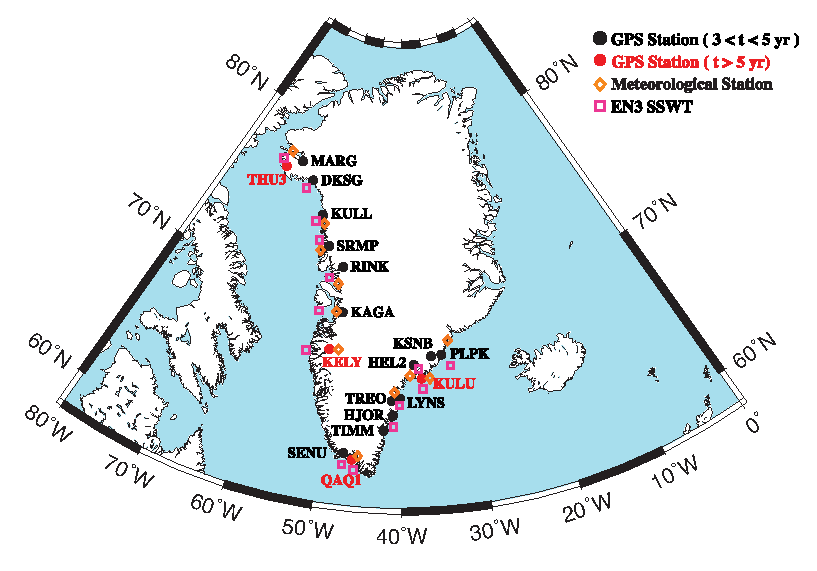
\includegraphics{figs_chpt3/2012GC004432-p01.eps} 
 \caption[Map of Greenland showing location of GPS sites, meteorological stations, and other data used in this study.]{Map of Greenland showing location of GPS sites, meteorological stations, and other data used in this study. Red circles indicate GPS sites with more than 5 years of data. Black circles indicate sites with 3 to 5 years of data. Orange diamonds indicate meteorological stations. Pink squares indicate pixels of sub-surface water temperature produced by EN3 model.}
 \label{fig:fig1}
\end{figure}

\clearpage
\begin{figure}
 \centering
 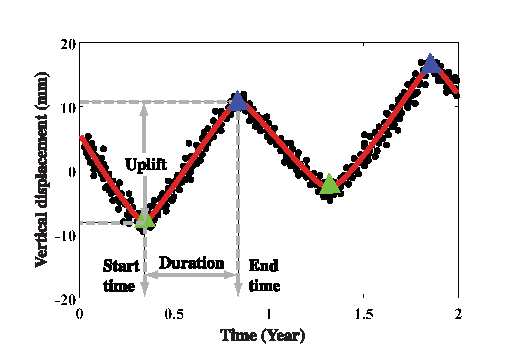
\includegraphics{figs_chpt3/2012GC004432-p02.eps} 
 \caption[Hypothetical 2 year time series showing four parameters (start time, end time, duration, and uplift) defined for a melt season.]{Hypothetical 2 year time series showing four parameters (start time, end time, duration, and uplift) defined for a melt season. Each black dot represents daily vertical position estimate. Red curve is best fit model. Blue triangles mark the maximum position value per year, and green triangles are the minimum value per year. A fifth parameter (rate of summer uplift) is the average slope of the curve between the start time and end time of uplift.}
 \label{fig:fig2}
\end{figure}

\clearpage
\begin{figure}
 \centering
 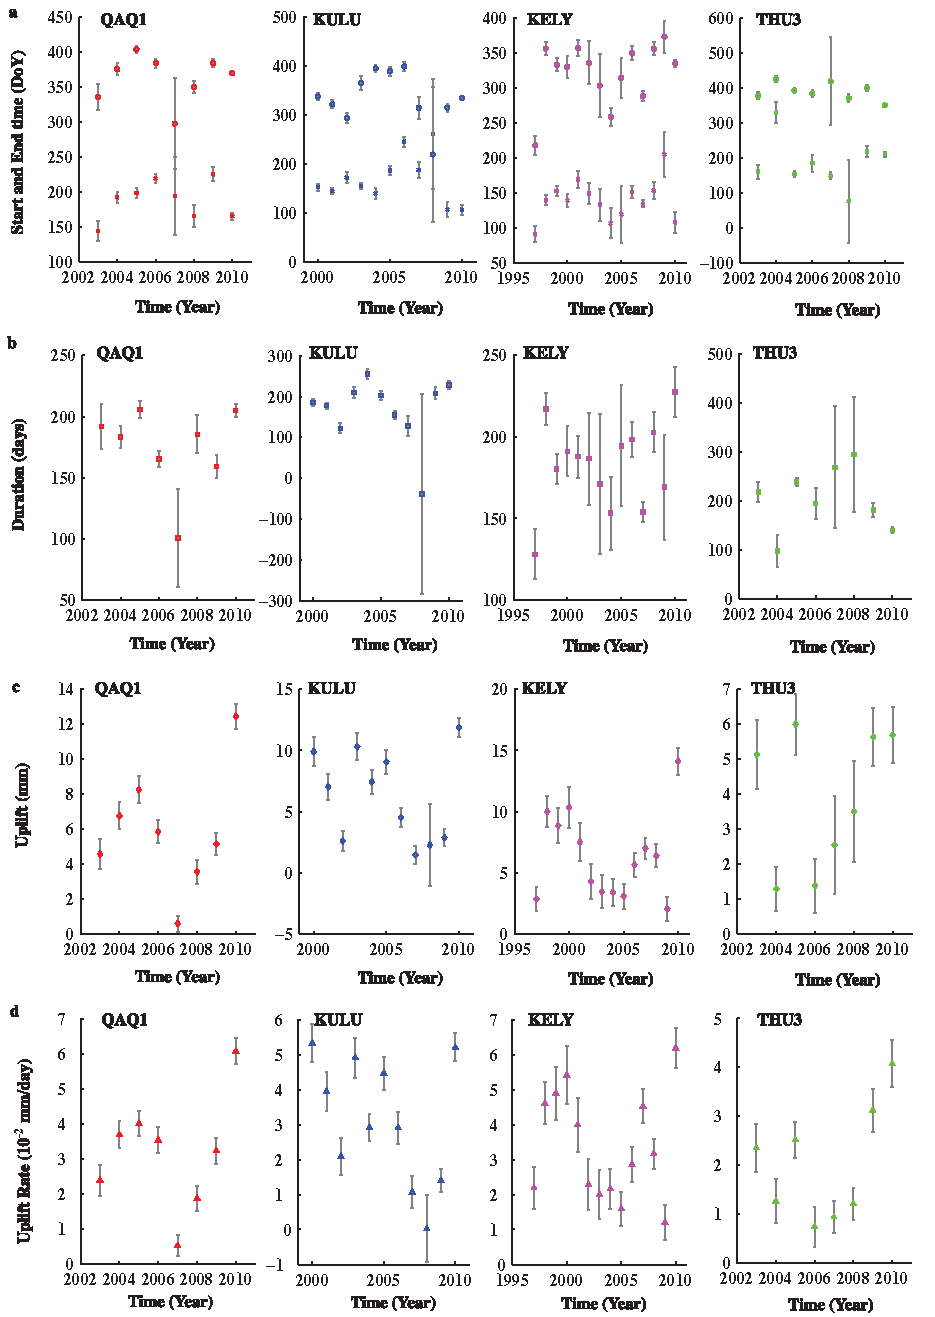
\includegraphics{figs_chpt3/2012GC004432-p03.pdf} 
 \caption[Annual variations of the five parameters defining seasonal uplift calculated for the four sites with longest observation record (red circles in Figure \ref{fig:fig1}).]{Annual variations of the five parameters defining seasonal uplift calculated for the four sites with longest observation record (red circles in Figure \ref{fig:fig1}). (a) Uplift start time (cross) and end time (circle), (b) uplift duration, (c) uplift magnitude, and (d) uplift rate. Gray line represents uncertainty.}
 \label{fig:fig3}
\end{figure}

\clearpage
\begin{figure}
 \centering
 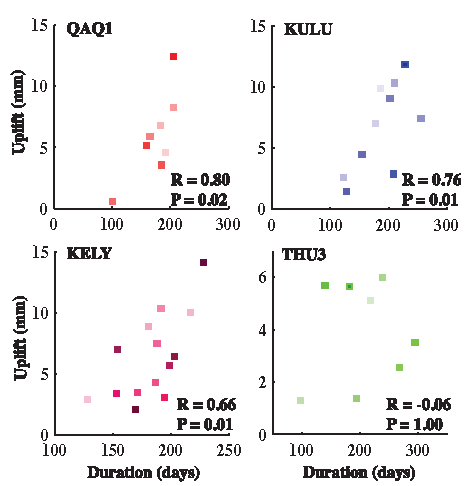
\includegraphics{figs_chpt3/2012GC004432-p04.pdf} 
 \caption[Uplift versus duration for the four sites with longest observation record.]{Uplift versus duration for the four sites with longest observation record. Colors varying from light to dark represent data from earlier to more recent.}
 \label{fig:fig4}
\end{figure}

\clearpage
\begin{figure}
 \centering
 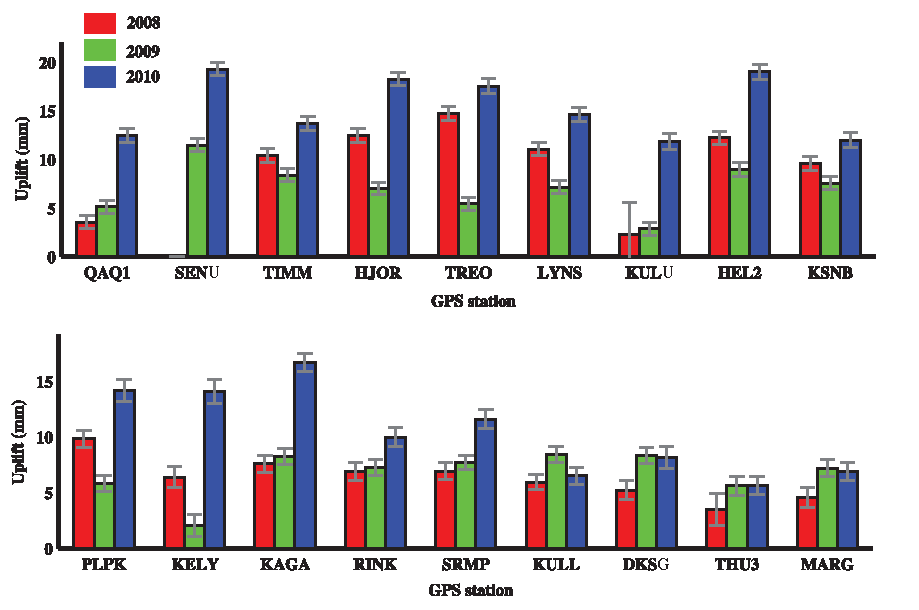
\includegraphics{figs_chpt3/2012GC004432-p05.pdf} 
 \caption[Seasonal uplift patterns for 2008–2010.]{Seasonal uplift patterns for 2008–2010. GPS sites are ordered by latitude, from south to north. Note change between KAGA (69.2 \textordmasculine N) and RINK (71.9 \textordmasculine N) with lower amplitude and lower variability uplift at the more northern sites.}
 \label{fig:fig5}
\end{figure}

\clearpage
\begin{figure}
 \centering
 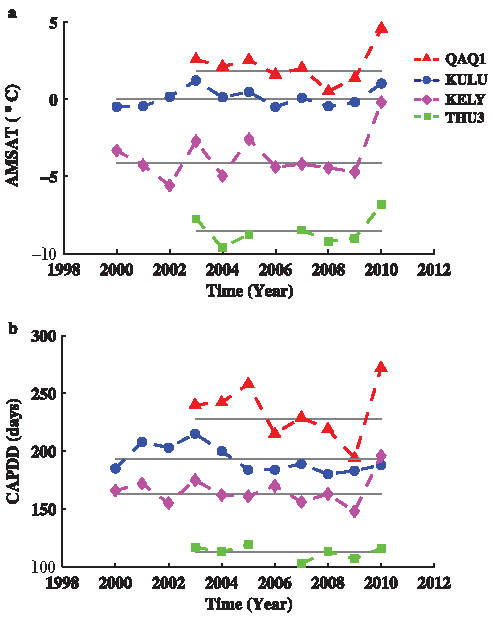
\includegraphics{figs_chpt3/2012GC004432-p06.pdf} 
 \caption[(a) AMSAT (Annual mean surface air temperature). (b) CAPDD (Cumulative annual positive degree days) for the four GPS stations with longest observation record.]{(a) AMSAT (Annual mean surface air temperature). (b) CAPDD (Cumulative annual positive degree days) for the four GPS stations with longest observation record. Solid gray line represents the mean value of reference period.}
 \label{fig:fig6}
\end{figure}

\clearpage
\begin{figure}
 \centering
 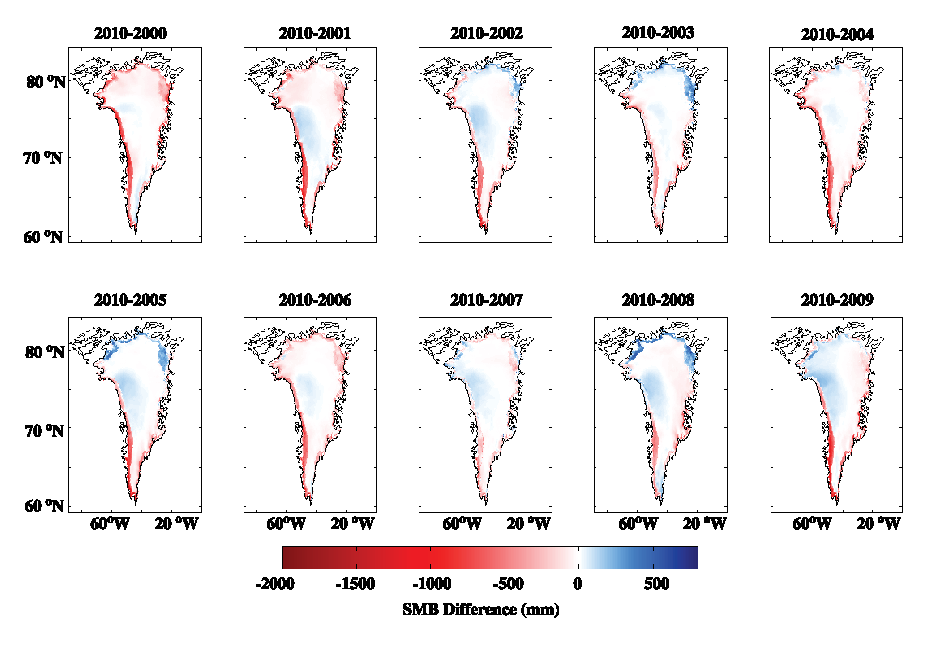
\includegraphics{figs_chpt3/2012GC004432-p07.eps} 
 \caption[Difference of Surface Mass Balance (SMB model from RACMO2) in summertime (June to August) between 2010 and 20XX (XX= 00–09) for the Greenland region.]{Difference of Surface Mass Balance (SMB model from RACMO2) in summertime (June to August) between 2010 and 20XX (XX= 00–09) for the Greenland region. Red color indicates that 2010 had a relatively negative SMB (more surface mass loss or less surface mass gain) compared to previous years, and blue color indicates that 2010 had a relatively positive SMB (less surface mass loss or more surface mass gain) compared to previous years.}
 \label{fig:fig7}
\end{figure}

\clearpage
\begin{figure}
 \centering
 \includegraphics{figs_chpt3/2012GC004432-p08.eps} 
 \caption[Difference of AMSSWT (Annual mean, sub-surface water temperature, depth range 5 m – 447 m) between 2010 and 20XX (XX = 00–09) for the Greenland region.]{Difference of AMSSWT (Annual mean, sub-surface water temperature, depth range 5m – 447 m) between 2010 and 20XX (XX = 00–09) for the Greenland region. Warmer colors indicate that 2010 was warmer than the previous year at a given location.}
 \label{fig:fig8}
\end{figure}

\clearpage
\begin{figure}
 \centering
 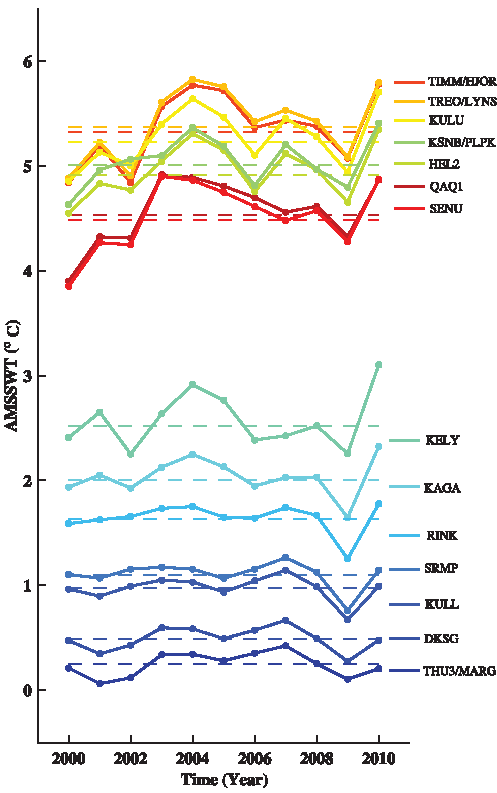
\includegraphics{figs_chpt3/2012GC004432-p09.pdf} 
 \caption[AMSSWT (Figure \ref{fig:fig8}) for “voxels” (model volume elements) nearest a given GPS station.]{AMSSWT (Figure \ref{fig:fig8}) for “voxels” (model volume elements) nearest a given GPS station. Warmer colors indicate southern latitudes, cooler colors indicate northern latitudes. Dashed color line represents 2000–2009 means. Note the pronounced 2010 anomaly for most locations, decreasing in intensity to the north.}
 \label{fig:fig9}
\end{figure}

\clearpage
\begin{figure}
 \centering
 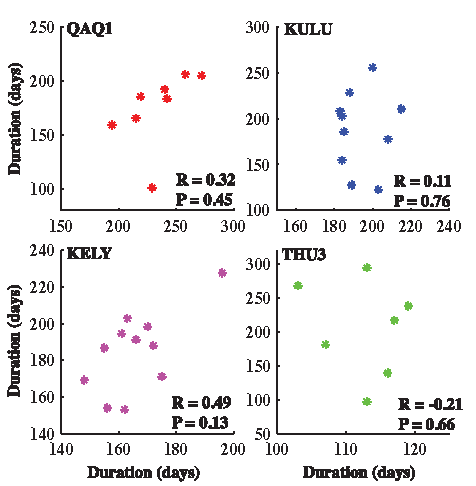
\includegraphics{figs_chpt3/2012GC004432-p10.pdf} 
 \caption{Uplift duration versus CAPDD (Figure \ref{fig:fig6}).}
 \label{fig:fig10}
\end{figure}

\clearpage
\begin{figure}
 \centering
 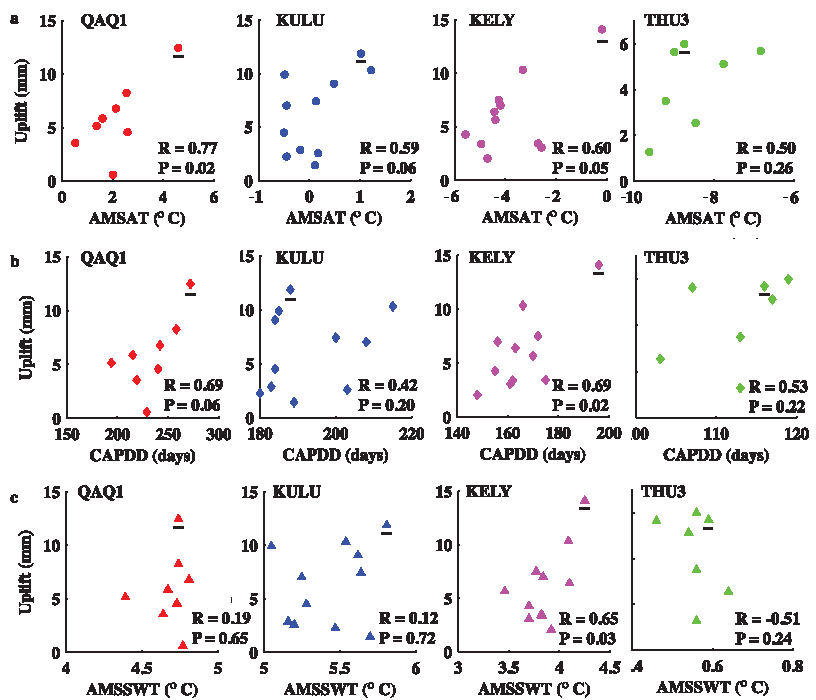
\includegraphics{figs_chpt3/2012GC004432-p11.pdf} 
 \caption[Spatial variation of seasonal uplift for four stations with longest time span related to (a) AMSAT (Figure \ref{fig:fig6}); (b) CAPDD (Figure \ref{fig:fig6}); and (c) AMSSWT (Figure \ref{fig:fig8}).]{Spatial variation of seasonal uplift for four stations with longest time span related to (a) AMSAT (Figure \ref{fig:fig6}); (b) CAPDD (Figure \ref{fig:fig6}); and (c) AMSSWT (Figure \ref{fig:fig8}). Underlined symbol is 2010.}
 \label{fig:fig11}
\end{figure}

\clearpage
\begin{figure}
 \centering
 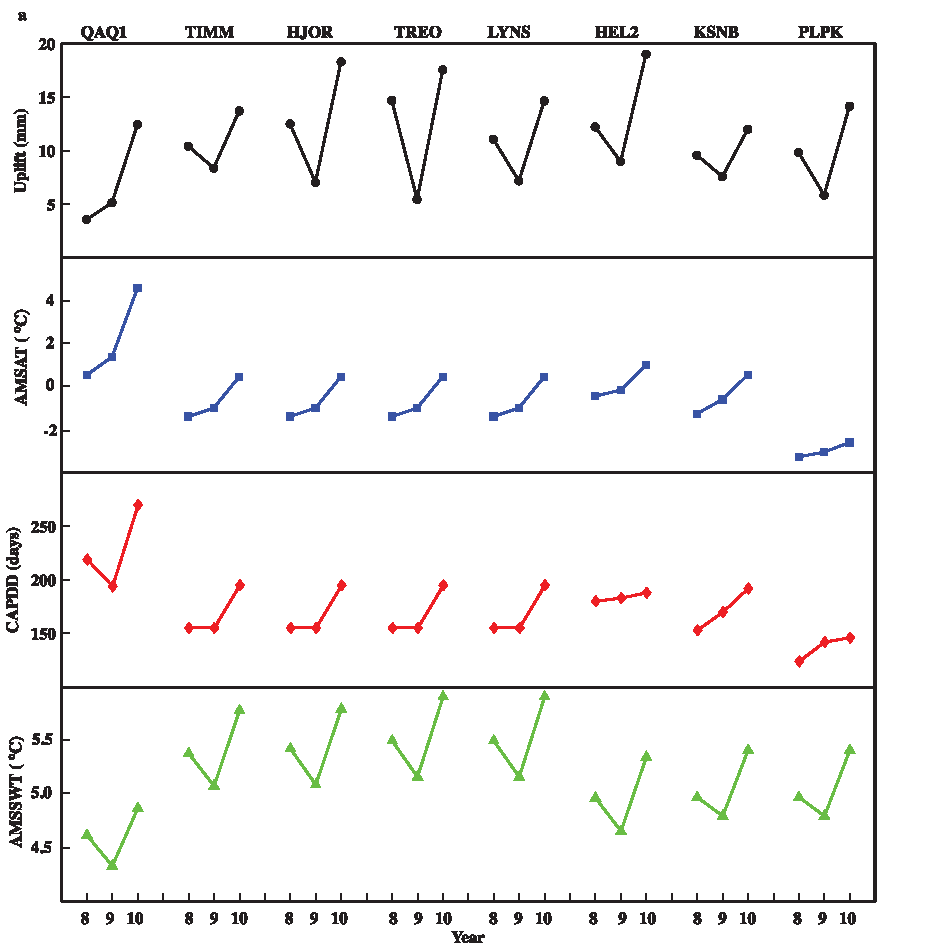
\includegraphics{figs_chpt3/2012GC004432-p12a.pdf} 
\end{figure}

\begin{figure}
 \centering
 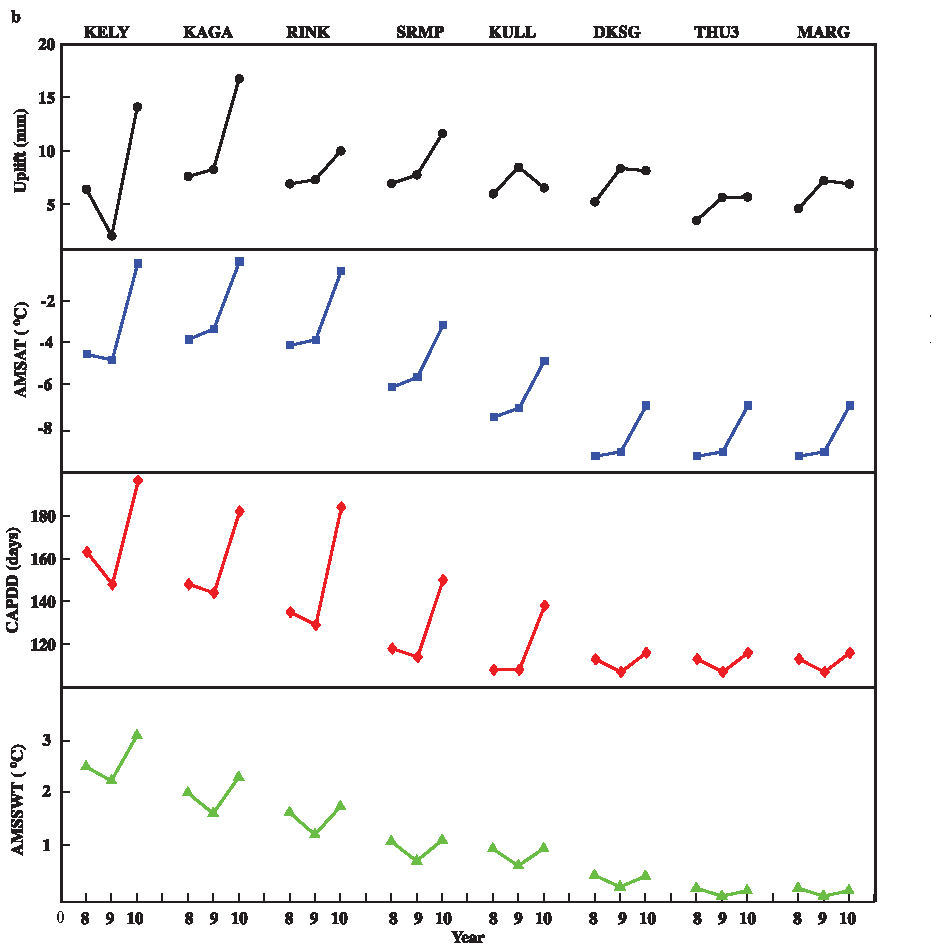
\includegraphics{figs_chpt3/2012GC004432-p12b.pdf} 
 \caption[Comparison between seasonal uplift patterns and atmospheric parameters (AMSAT and CAPDD, Figure \ref{fig:fig6}) as well as the ocean temperature parameter (AMSSWT, Figure \ref{fig:fig8}) for 2008–2010.]{Comparison between seasonal uplift patterns and atmospheric parameters (AMSAT and CAPDD, Figure \ref{fig:fig6}) as well as the ocean temperature parameter (AMSSWT, Figure \ref{fig:fig8}) for 2008–2010. Uplift pattern as shown in Figure \ref{fig:fig5}. SENU and KULU are eliminated here due to lack of data in 2008. GPS stations are ordered from south to north.}
 \label{fig:fig12}
\end{figure}

\clearpage
\begin{figure}
 \centering
 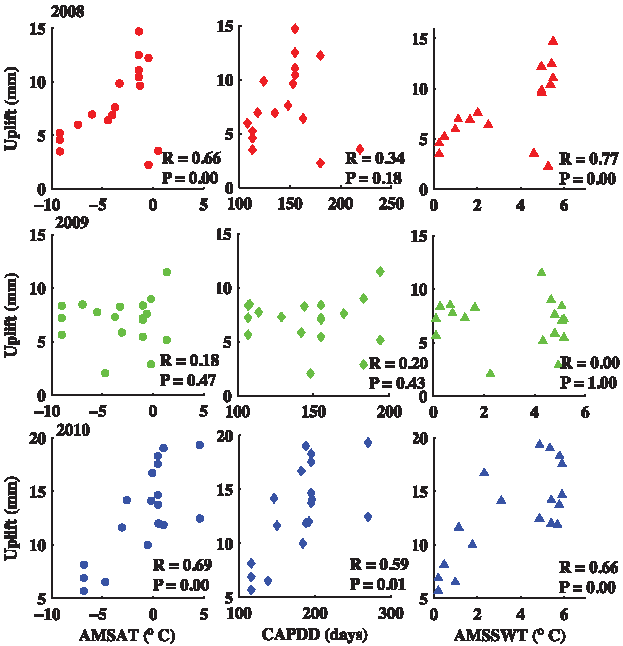
\includegraphics{figs_chpt3/2012GC004432-p13.pdf} 
 \caption{Temporal variation of seasonal uplift for all stations for 2008–2010 as a function of AMSAT
(Figure \ref{fig:fig6}), CAPDD (Figure \ref{fig:fig6}), and AMSSWT(Figure \ref{fig:fig8}).}
 \label{fig:fig13}
\end{figure}

\clearpage
\begin{figure}
 \centering
 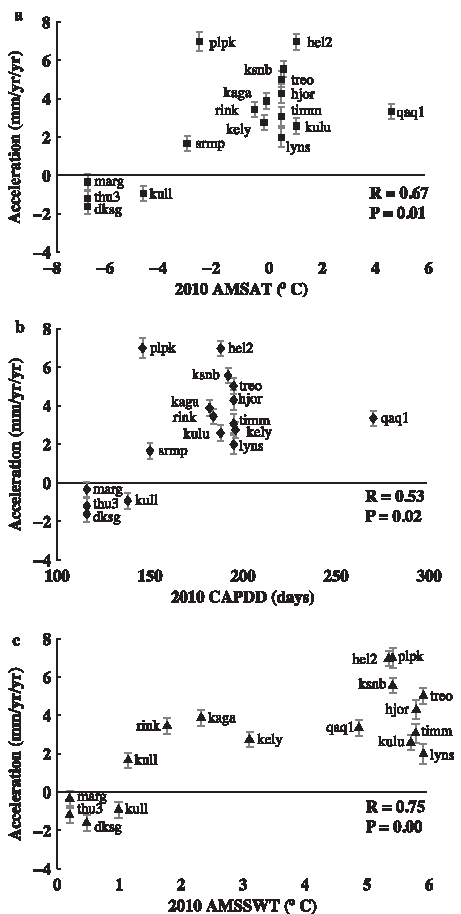
\includegraphics{figs_chpt3/2012GC004432-f14.pdf} 
 \caption{Spatial variation of uplift accelerations as a function of (a) AMSAT (Figure \ref{fig:fig6}), (b) CAPDD (Figure \ref{fig:fig6}), and (c) AMSSWT (Figure \ref{fig:fig8}) of 2010.}
 \label{fig:fig14}
\end{figure}

\clearpage
\begin{figure}
 \centering
 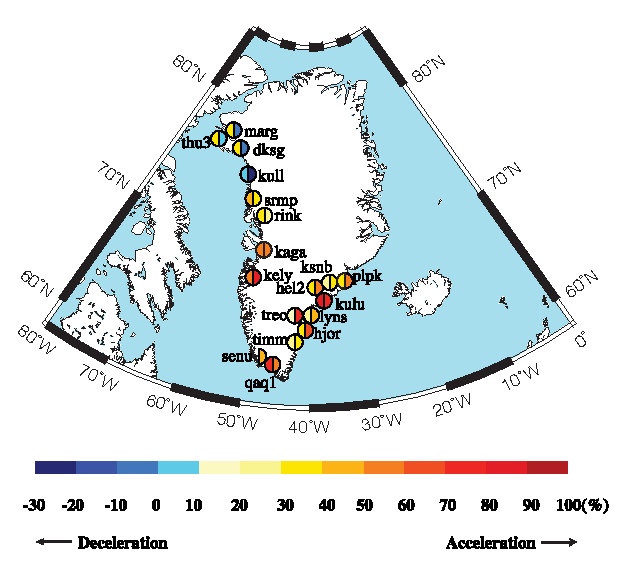
\includegraphics{figs_chpt3/2012GC004432-p15.pdf} 
 \caption[Site map of relative difference between uplift in 2010 and uplift in 2008 and 2009.]{Site map of relative difference between uplift in 2010 and uplift in 2008 and 2009. The left half circle shows percentage difference between the uplift in 2008 and 2010: $\triangle$U$_{10/08}$ = (U$_{10}$ - U$_{08}$)/U$_{10}$; right half circle shows percentage difference between uplift in 2009 and 2010: $\triangle$U$_{10/09}$ = (U$_{10}$ - U$_{09}$)/U$_{10}$.}
 \label{fig:fig15}
\end{figure}

\clearpage
\begin{figure}
 \centering
 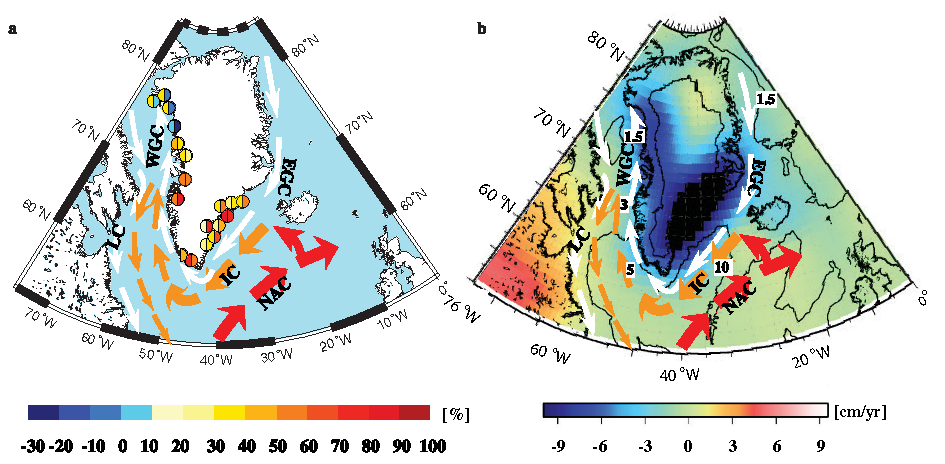
\includegraphics{figs_chpt3/2012GC004432-p16.pdf} 
 \caption[Relation between ocean currents, coastal uplift, and ice mass balance of coastal Greenland.]{Relation between ocean currents, coastal uplift, and ice mass balance of coastal Greenland. Red arrows indicate the mean path of the warm North Atlantic Current (NAC); orange arrows indicate Irminger Current (IC), white arrows indicate East Greenland Current (EGC), West Greenland Current (WGC) and Labrador Current (LC). (a) Relative difference between uplift in 2010 and that in 2008 and 2009 as shown in Figure 15. Names of GPS stations were omitted here. (b) Mass loss in equivalent water height over Greenland between February 2003 and January 2008 observed by GRACE \cite[]{wouters2008grace}. Numbers indicate the mean temperature (\textordmasculine C) of Atlantic-sourced waters on the Greenland shelf \cite[]{straneo2012characteristics}.}
 \label{fig:fig16}
\end{figure}